\documentclass[twocolumn]{jsarticle}
\usepackage[dvipdfmx]{graphicx}
\usepackage{mathrsfs,calligra,calrsfs,url,bm,here,caption}
% \captionsetup[table]{labelsep=period,justification=raggedright, singlelinecheck=off}
\usepackage{aic2022}
\title{AIC Databricks プロジェクト}
\author{西川誠人$^1$,勝又圭$^2$,好田駿成$^3$}
\affiriation{$^1$慶應義塾大学大学院理工学研究科\\$^2$慶應義塾大学理工学部情報工学科\\$^3$慶應義塾大学経済学部}
\abst{\\
昨今,ビジネスにおいてビッグデータを活用する取り組みが広く行われている.一方で,データ活用のためには相応のデータ基盤が必要になるため,
人材やノウハウの無い企業においてはデータ活用が遅れている.この現状に対し,企業にデータ活用プラットフォームを提供するサービスが生まれている.
我々は,このようなサービスの1つである,Databricksについて調査し,AICの講習会を行うことを目的に活動している.
本ポスターではこれまで我々が行ってきた調査内容についての発表を行う.
}
\keywords{Databricks, Machine Learning, Datawarehouse, AI, Open Source}
\begin{document}
\maketitle
\section{研究背景・目的}
2022年度のAIC新設のプロジェクトとして,新しいAI/Data Science PlatformであるDatabricksの調査・評価プロジェクトが2022年6月からスタートした。
Databricksとはデータの収集・蓄積から分析・機械学習モデル開発並びに運用を一気通貫・効率的かつ安価に行うことができるオープンソースの統合プラットフォーム\cite{databricksHP}である。
機械学習・AIが注目される昨今だが、情報インフラ構築の難易度やノウハウの欠如からデータ活用ができていない企業も多く、機械学習エンジニアの雇用・分析環境の構築の観点から機械学習の大規模な活用は大企業にとどまることがほとんどである。
今回の調査対象であるDatabricksを提供するDatbricks社はデータとAIの民主化を掲げ、機械学習等のデータ活用を大企業以外にも活用できるようにノウハウを持たない企業におけるデータ活用を推進している。
DatabricksはGartnerの2022年「クラウドデータベース管理システム(CDBMS)部門のマジック・クアドラント」において、2年連続でリーダーの1社\cite{Gartner}として位置付け今後のDe Fact Standard化が期待されている。
そんなDatabricksについて学生視点から分析を行い、慶應義塾大学内での活用可能性やDatabricksを学ぶことの意義を評価することが本プロジェクトの目的である。
\section{方法}
本プロジェクト実施にあたりDatabricksの提供手法の一つであるDatabricks On AWSを使用した。他のクラウドプラットフォームとしてGoogle Cloud Platform, Microsoft Azure等が挙げられるが、
実際にDatabricksが活用されている企業の中で一番使われていること、Databricks社が2022年8月に実施したDatbricks Hands Onにて使用されていたことなどからAWSを選択した。\par 
調査方法は主に以下の手順によって実施した。
\begin{enumerate}
  \item Databricks社の提供するHands On への参加
  \item Databricks社が提供する学習コンテンツDatabricks Learningを用いた学習の実施
  \item オープンデータを用いた自由なDatabricksのデータ分析の実施
  \item 他の類似サービスとの比較・優位性の調査
\end{enumerate}
以上の手順によりDatabricksの学習コスト、他のプラットフォームを使用した際と比較したデータ分析のしやすさを評価した。
\section{Databricksについて}
\subsection{サービスアーキテクチャ}
\subsubsection{レイクハウスとは}
\begin{figure}[H]
  \centering
  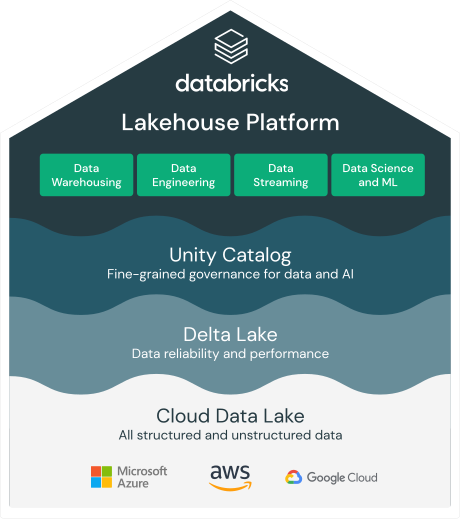
\includegraphics[width=6cm]{./image/Marketecture.png}
  \caption{レイクハウスプラットフォーム概略図}
  \label{lakehouse}
  \title
\end{figure}
Databricksでは新たなデータ活用プラットフォームの形としてレイクハウスを提案している。
レイクハウスとはデータウェアハウスと多様なデータを単一のシステムで活用するためのデータレイクそれぞれの利点を組み合わせたアーキテクチャである。
一般に古くから用いられるデータウェアハウスは近年の機械学習の発達により活用が促進されている画像や音声などの非構造化データの格納には適しておらず、データレイクはトランザクション・データ品質の保証等に適していないという課題があった。
これらの課題を解決するのがレイクハウスであり、データウェアハウスと同様のデータ構造とデータ管理能力を搭載している他、データレイクのメリットである低コストなストレージへの直接アクセスを実現している。
構造化データは勿論、非構造化データ等のさまざまなデータタイプが格納できるほか、トランザクションやBI、様々な言語が同一のノートブックで使用できるなど他のプラットフォームと比較した優位性があるといえる。DatabricksにおけるレイクハウスプラットフォームはFig1のように構成されており、DatabricksでレイクハウスはDelta Lakeと呼ばれるOSSで実現されている。

% Fig.\ref{lakehouse}
\subsubsection{インフラ}
Databricksで用いられるインフラ構築は一括で各クラウドプラットフォームをもとに行われている。DatabrickではMicrosoft Azure、Amazon Web Servbices、 Google Cloud Platformの3種のクラウドに対応しており、それぞれのインフラ管理についてもDatabricks専用のGUIによって管理可能である。
ノウハウが少ない中小企業での活用を目的としていることもあり、Databricksに必要な機能に絞った構成となっており、各クラウドから自力で環境構築するより容易であり学習コストも低い。
\subsection{主要機能}
Databricksでは主にData Science \& Engineering、Databricks SQL、Databricks Machine Learningの3つの機能から構成されている。
\subsubsection{Data Science \& Engineering}
Data Science \& Engineeringはデータの取得・加工を目的としたApache Sparkを中心として基づくデータ分析プラットフォームである。
HTML等を用いた機能実装による非エンジニア人材のデータ利用の促進が可能など、データエンジニア・データサイエンティスト等社内のさまざまな人材間のデータコラボレーションが可能なプラットフォームである。
使用感としてはJupyter NotebookやGoogle Colabratory等と似ており、Databricksを初めて使用するユーザーであっても親和性の高いデザインであることが魅力である。
\begin{figure}[H]
  \centering
  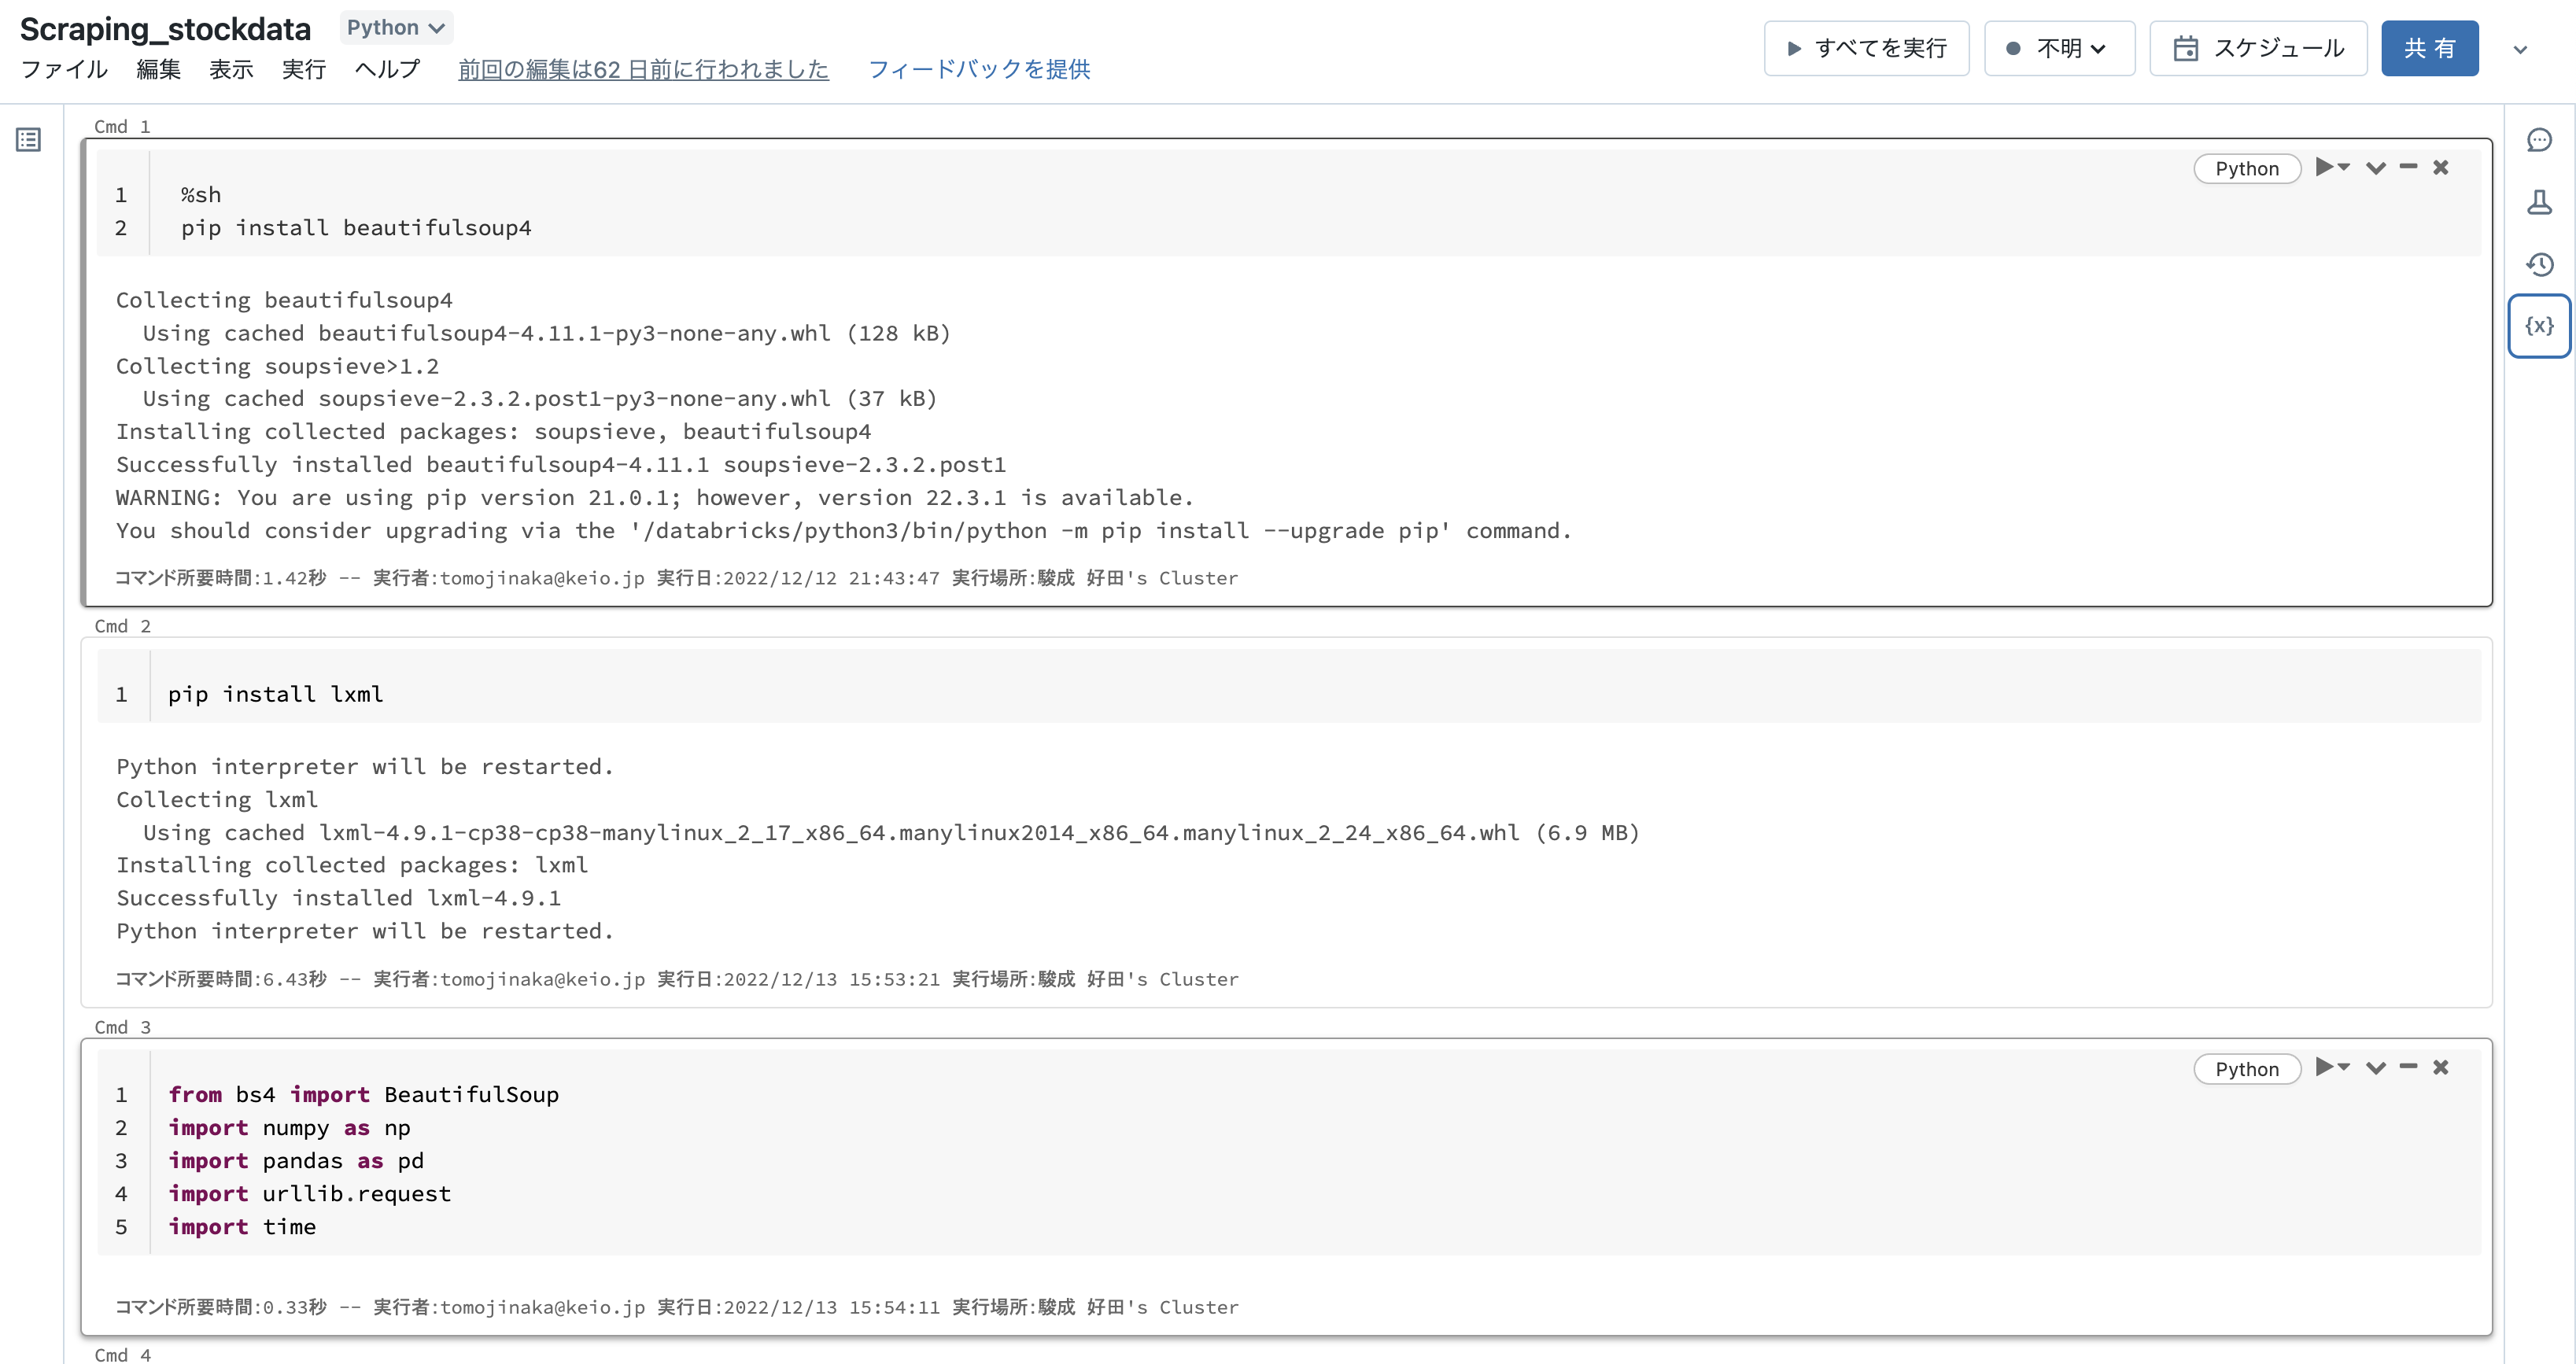
\includegraphics[width=8cm]{./image/notebook.png}
  \caption{Notebook 使用画面}
  \label{Notebook}
  \title
\end{figure}
ETL(Extract/Transform/Load)のためのインフラとしてさまざまなOSSから構成されており、特にSpark Core APIが導入されていることでR、SQL、Python、Scala、Javaを宣言一つで切り替えられるのは他のプラットフォームにはない魅力と言える。
各ファイルはNotebookと呼ばれ、このNotebook単位でジョブを定義でき、定期実行やパイプラインの作成がGUIからも容易に設定が可能で定期的に保存されるデータの継続的な加工に適している。
また、各ノートブックの運用環境としてApache Spark クラスターが用いられ、GPU・CPU性能を容易にスケールアップ/スケールダウンでき、その設定も共有できる点も魅力的だ。
\subsubsection{Databricks SQL}
Databricks SQLでは、SQL開発者がETL、分析、ダッシュボードの作成を行うための一連のツールが用意されているコンポーネントである。
BIツールと直結したデータウェアハウスでのダッシュボードが作成可能のため、ダッシュボード反映までのスピードが早い点が魅力。
SQL の実行結果をワンクリックで可視化ができ、直感的なダッシュボード構築など非エンジニアなデータアナリストへの配慮が多くなされている。
Data Science \& Engineeringのクラスターと同様にSQLウェアハウスと呼ばれる実行環境が用意されており、クラスター同様に必要度に応じてスケールアップ/スケールダウンを容易に実現可能である。
また、BIツールの必要に応じてDatabricksではLookerをは始めとしてさまざまなサードパーティー製のツールとの連携ができ、可視化のためのダッシュボード作成にはさまざまな手段が用意されている。
\begin{figure}[H]
  \centering
  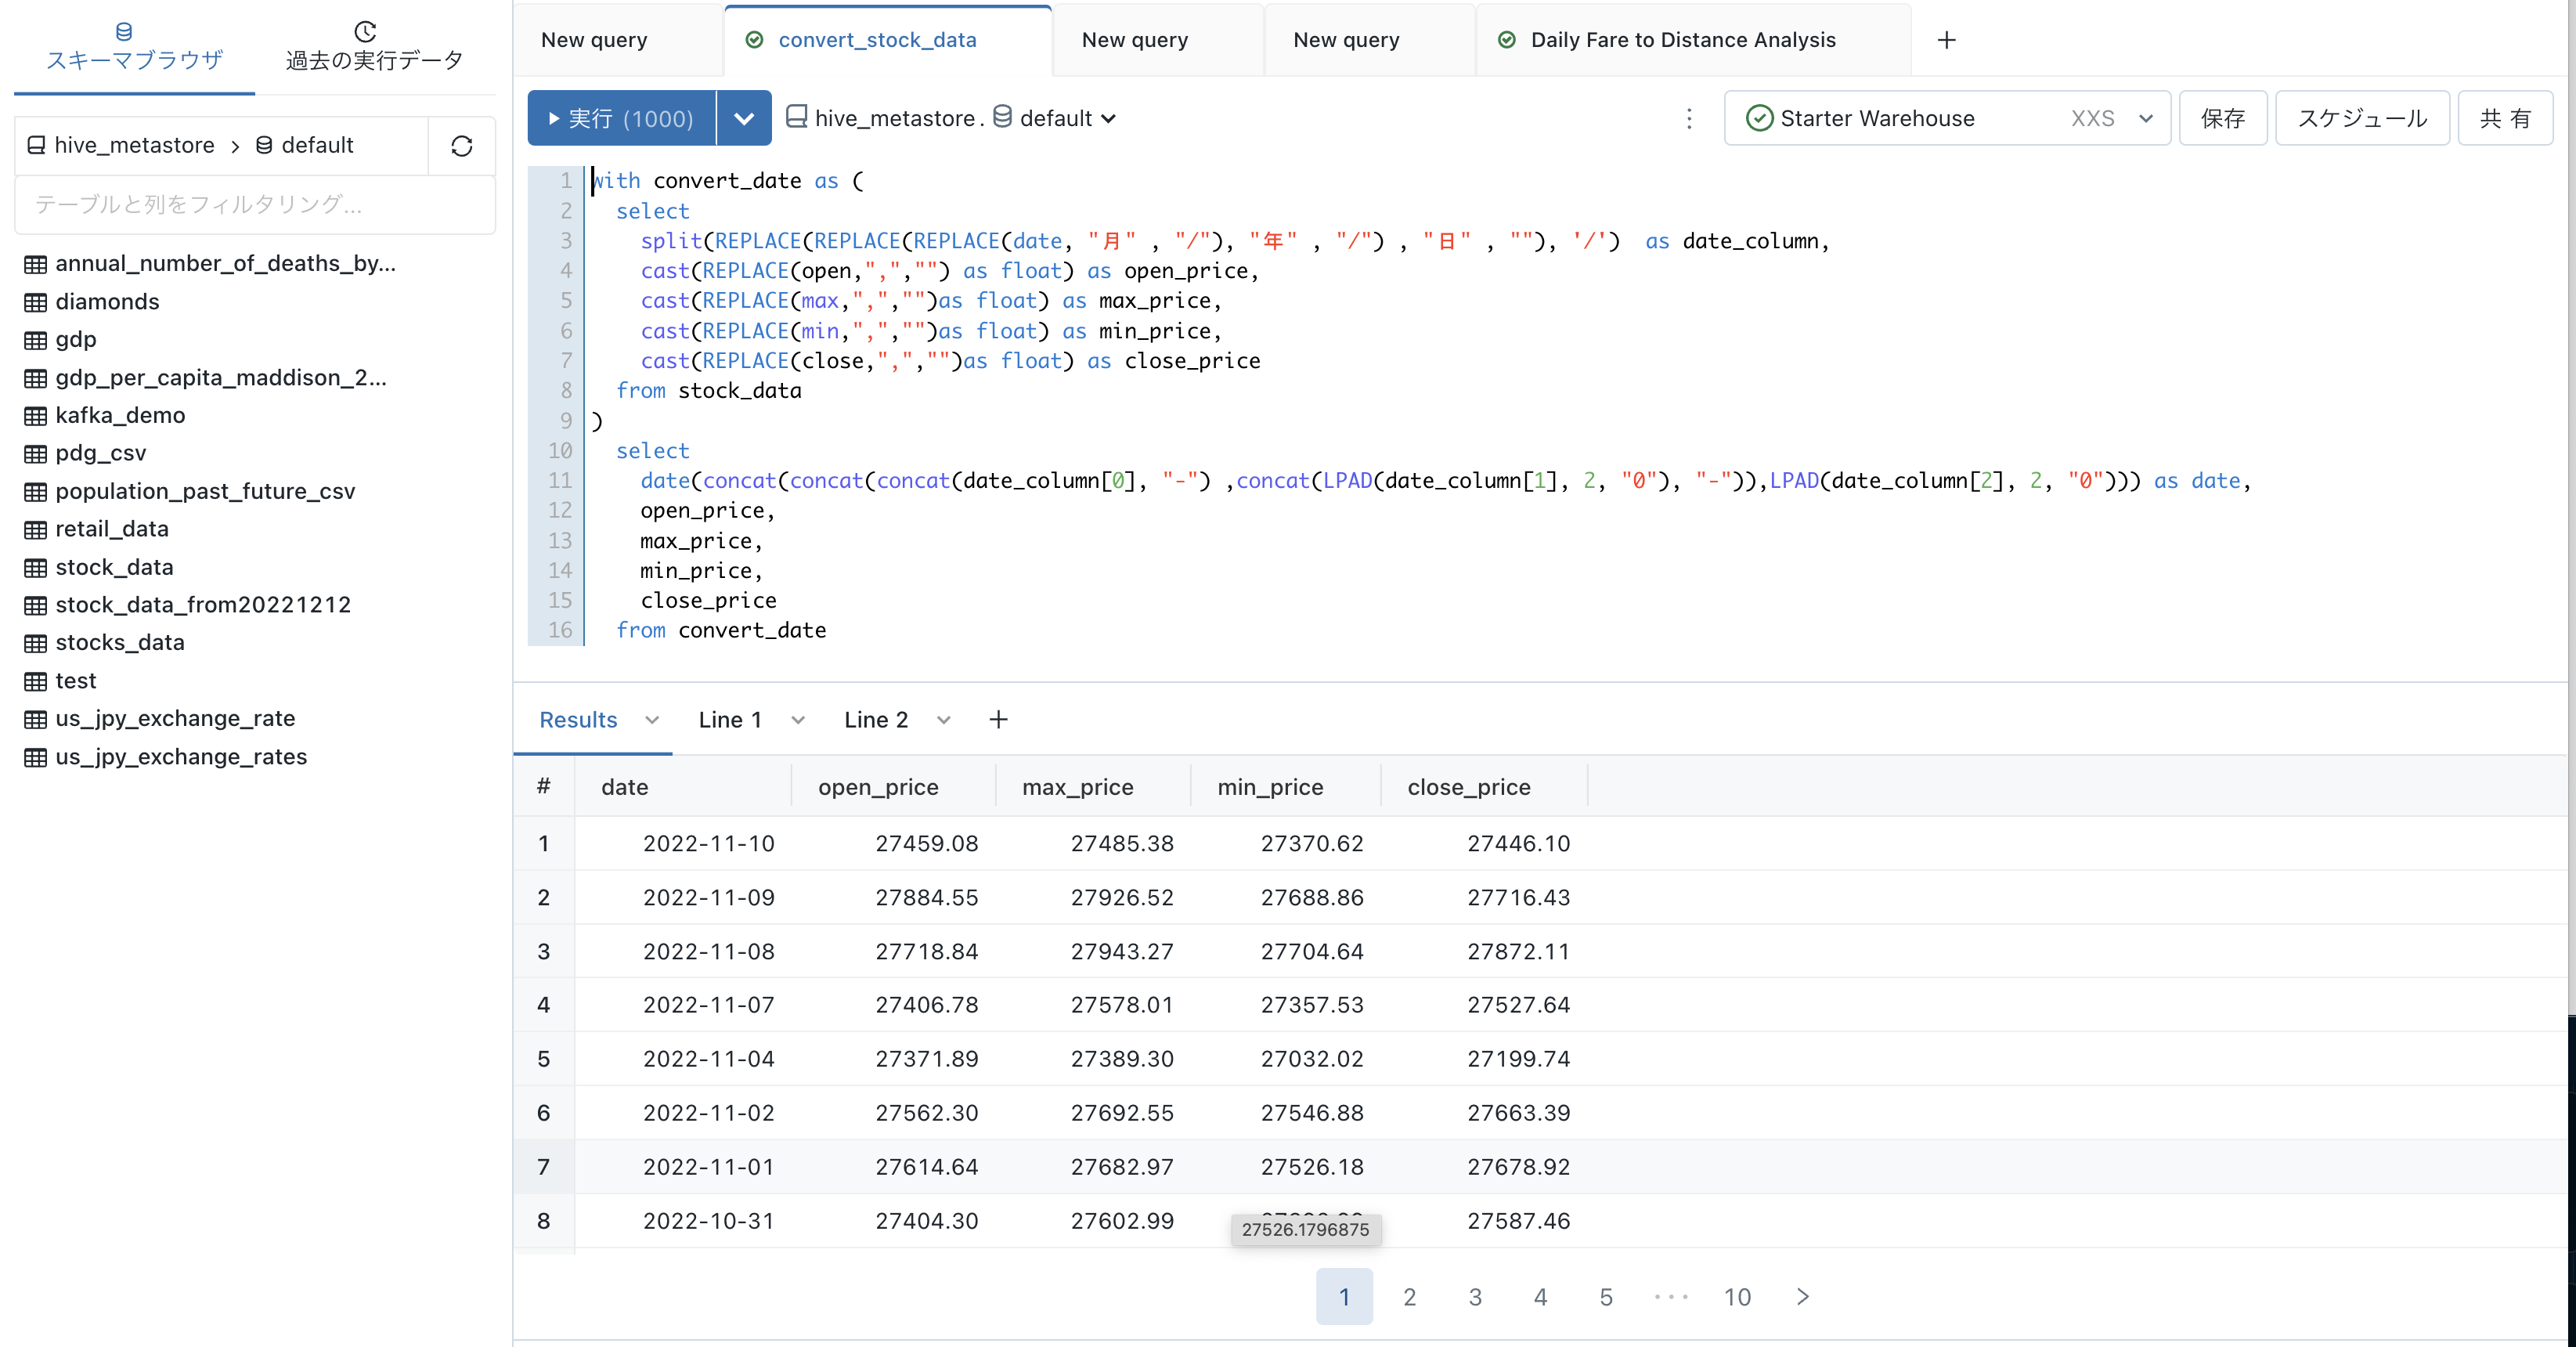
\includegraphics[width=8cm]{./image/SQL.png}
  \caption{Databricks SQL Query 使用画面}
  \label{SQL}
  \title
\end{figure}
\begin{figure}[H]
  \centering
  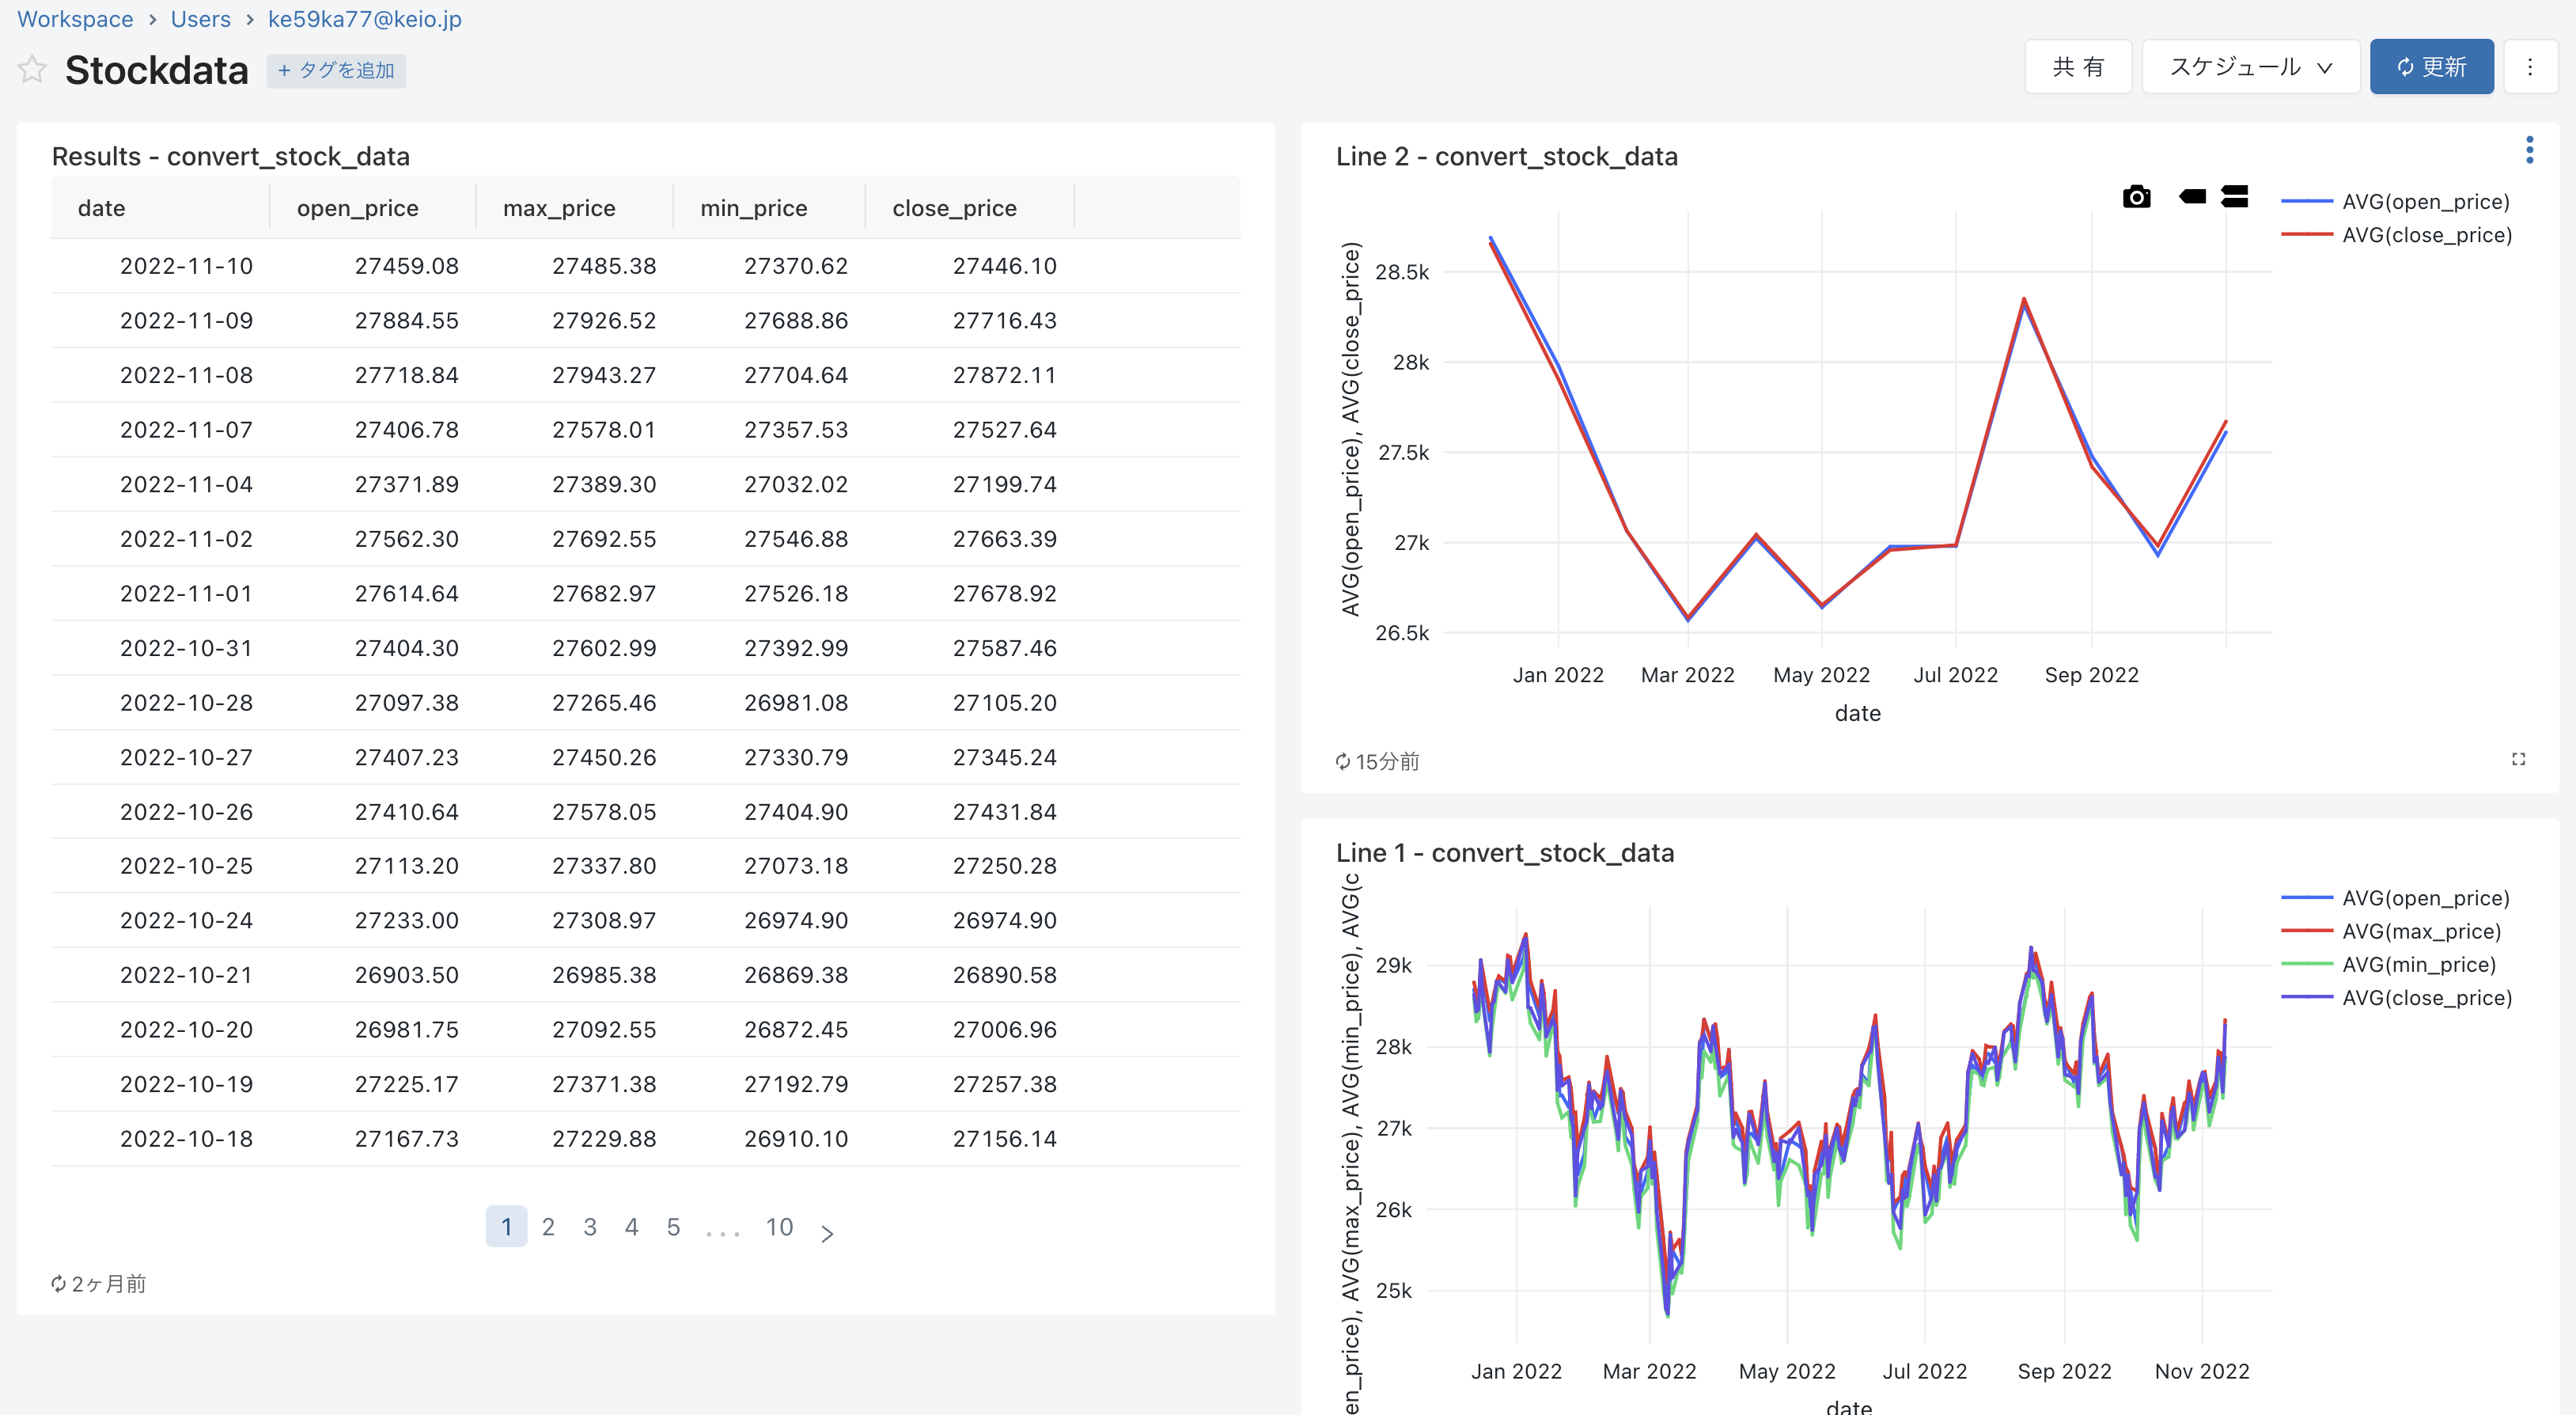
\includegraphics[width=8cm]{./image/dashboard.png}
  \caption{Databricks SQL Dashboard 使用画面}
  \label{Dashboard}
  \title
\end{figure}
\subsubsection{Databricks Machine Learning}
Databricks Machine Learningとは機械学習のモデル作成においてそのトレーニングの過程の追跡や管理を行うための機械学習プラットフォームである。
主に先述のData Science \& EngineeringのNotebookを用いてデータ加工、学習を行うおこなう。機械学習モデルの作成のため、Databricks Macine Learningでは
モデルの自動作成のためのAuto ML、ハイパーパラメーターチューニングを行うためのモデルのトレーニング状況を追跡を行うML Flowを用いた実験(Experiment)機能、モデルの共有・管理・提供のためのモデルレジストリがこのコンポーネントでは提供されており、
自前の環境では環境構築の難易度が高い機械学習向けインフラを容易に使用できるエンドツーエンドのプラットフォームである。
\begin{figure}[H]
  \centering
  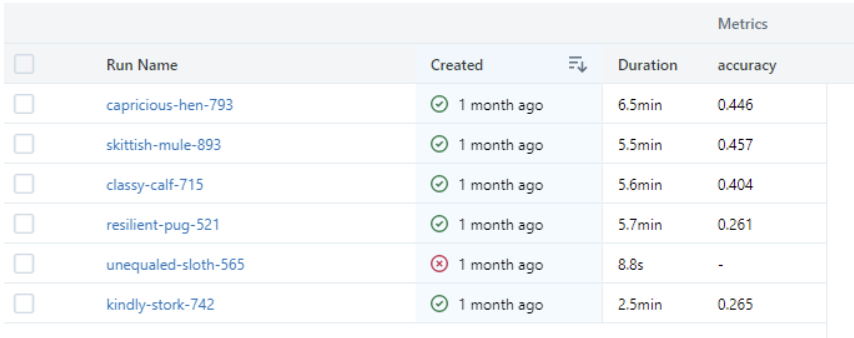
\includegraphics[width=8cm]{./image/storing.png}
  \caption{Databricks Machine Learning モデルレジストリ}
  \label{Storing}
  \title
\end{figure}
\begin{figure}[H]
  \centering
  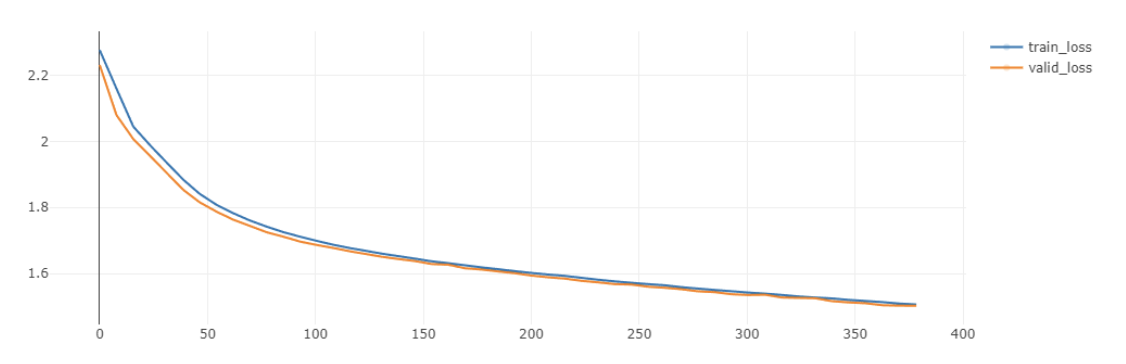
\includegraphics[width=8cm]{./image/showing.png}
  \caption{Databricks Machine Learning 実験(Experiment)}
  \label{showing}
  \title
\end{figure}
\section{調査結果}
\subsection{Databricksの強み}
前節までの調査をもとにDatabricksの強みをまとめる。
まず第一にデータ活用に必要な機能が一通り揃っている環境をブラウザ上で容易に使用できる点が挙げられる。
Datbricksを用いれば先述の諸機能を利用してデータ収集からMLモデル運用までを一気通貫に同一プラットフォーム上で行うことが可能である。
また、GUIで容易に操作が可能なUI設計がされており、機能間での連携に詳しい知識がいらない点も魅力的と言える。\par
第二にコスト面である。DatabricksはOSSのアプリケーションであるため、個々の機能がマネージドサービスとして提供されており、分析基盤の維持管理が不要である。従って、大きく事業者にのしかかるメンテナンスコストの削減が見込める。
また、クラウドインフラのリソース (コスト) 管理が容易であり、オンプレミスで環境を用意する場合と比較して事業の成長度合いやプロジェクトの進捗により規模のスケールアップ/スケールダウンが容易に変更できるkとおは大きな魅力だ。
第三に非エンジニアでも使えるUI設計がある。Notebook、SQL Query、Dashboardに至るまで非エンジニアが利用することを想定したUI設計がされており、エンジニア側でも機能拡張の伸び代も大きいなどチームでの利用にとても親和性が高いプラットフォームと言える。
煩雑なクラスターの設定など低レイヤの技術が隠蔽されていることで初心者や非エンジニアにとっても利用しやすく、データ分析に対するネガティブな印象を減らすことができるほか、直感的に使用可能なUIにより学習コストも削減できる。
以上のような理由から組織でのビジネスには非常に強力なツールであると言える。
\subsection{大学内での使用可能性評価}
前述の内容を考えると学生にとってDatabricksがオーバースペックであることは否めないことは確かだ。一方で本プロジェクトメンバーではアカデミアでDatabricksは無価値とは考えていない。
慶應義塾大学におけるユースケースを考察すると学生の個人利用と授業や研究活動の主に二分されると考える。
まず、学生のDatabricksの個人利用だが、純粋にデータ解析のみを行いたい学生には有用なツールと言える。今後De Facto Standardになりうるツールを学ぶことは社会に出てから役立つといえ、学生向け無償プランも提供されている点からも導入する価値は高い。
Databricksには先述の通り多様なOSSによりデータ分析における様々な機能が格納されている。Databricksをデータ分析のプラットフォームとして利用するもよし、参考にOSSへの知見を深めるのもよし、各種技術の学習きっかけにもなり得るツールである。
授業や研究活動において「非情報系だがデータ解析を行う」ような研究や授業では有用であると言える。もちろん情報系の研究室でデータ解析自体を研究対象としている研究室であればオンプレミスの開発環境を所持していることが多く必要性は薄い。
一方で機械学習を用いて別の分野の研究を行う研究室やプロジェクト、授業においてDatabricksを活用すれば環境構築・維持にかかる負荷の低減が実現でき、より本質的な議論へ時間を割くことができる。その時間の削減により新たな発展が生まれることを期待する。また、Databricksを用いることで最先端のデータ解析ツールを容易に用いることができ、
個人の開発環境では用いることのできない多様な機能によりより精度が高く、社会的価値の高い研究が多発生しうる機会を提供できるプラットフォームである。\par
\section{今後の展開}
本プロジェクトを通じてDatabricksの慶應義塾大学における利用可能性が高いことが評価できた。
様々な職種、特に非エンジニアでも使いやすいDatabricksというプラットフォームを利用して学習を進めることで、同様の内容を環境構築を含めて行なった場合と比較してデータ分析に挑戦することへの抵抗がなくなる可能性が期待できる。
また、すでにデータ分析等を既存のツールを使用しているエンジニアの学生に対しても手軽にデータ活用する方法を紹介し、将来のDe Facto Standardとなり得るDatabricksの学習を行うことは将来役立つ経験となることは確かだろう。
そして、OSS ベースで構築される ML インフラの全体像を掴むことで、データ分析基盤の全体像を知ることができ、現代社会で盛んに利用されているOSSという方式によるアプリケーション開発・活用の実態を知り、背後で稼動する OSS の挙動を考えながらシステムを触るきっかけとしたい。
以上のような理由からDatabricksを用いたハンズオンを中心として、Git, SQL等の関連技能の講習を含めた講習会をの実施を2023年春に企画している。
\section{結論}
本プロジェクトによりDatabricks社により提供されているDatabricksというデータ活用プラットフォームの有用性を評価することができた。ビジネス文脈で使用される機能を多く備えたツールであるという側面は理解した上で、
機械学習を使用することを目的として研究や学習用途で学生が使う有用性は大いに認められるだろう。AIC DatabricksプロジェクトとしてDatabricksの慶應義塾大学における普及・De Falcto Standard化を促進するため、Databricksに関する
授業提供を実施する。学生に機械学習が容易に活用できるという選択肢を提示することにより今後の慶應義塾大学での研究・学習における機械学習の活用が促進されることで未来の研究にポジティブに寄与してゆきたい。

\begin{thebibliography}{9}
  \bibitem{databricksHP}
  \bibitem{Gartner}
  \bibitem{QuickStartGuide}  クイックスタートガイド
  \bibitem{about_databricks} \url{https://learn.microsoft.com/ja-jp/azure/databricks/scenarios/what-is-azure-databricks-ws}
  \end{thebibliography}
\end{document}
%\label{lakehouse} $\url{https://www.databricks.com/jp/product/data-lakehouse}$]
